\documentclass{article}

\usepackage[main,final,nonatbib]{neurips_2026}
\usepackage[utf8]{inputenc}
\usepackage[T1]{fontenc}
\usepackage{hyperref}
\usepackage{url}
\usepackage{booktabs}
\usepackage{array}
\usepackage{graphicx}
\usepackage{xcolor}
\usepackage{amsmath}
\usepackage{arydshln}
\usepackage{float}
\usepackage{tikz}
\usetikzlibrary{arrows.meta,positioning}

\title{CSE/DSC 234 Project 2: Schema Linking with Supervised Fine-Tuning}
\author{Group 122 \\ Fengfei Yu (A69042700)}

\begin{document}
\clubpenalty=10000
\widowpenalty=10000
\displaywidowpenalty=10000
\maketitle

\begin{abstract}
This report describes a local schema-linking system for natural-language questions over relational
databases. Starting from 301 labeled examples, I converted each row into a compact schema prompt
and a structured JSON target, then upsampled low-resource databases to reduce the imbalance across
schemas. The final system fine-tunes a Qwen2.5-Coder 1.5B model with a LoRA adapter, uses
completion-only supervised fine-tuning, prunes the schema context before prompting, and filters
generated identifiers against the target schema. The experiments show a clear progression from a
weak no-SFT baseline to a stronger pruned, balanced, coder-model setup. The best development run
scored 0.6869 overall, with a table score of 0.7753 and a column score of 0.5985.
\end{abstract}

\section{Training Data Methodology}

The released training split contains 301 labeled examples. Each example has a question, a database
identifier, the gold SQL query, and the corresponding table and column links. I used these labeled
examples as the supervised training source. The released validation split was kept separate and used
only for model selection, error analysis, and reporting scores. I did not train on validation answers
or on unreleased SNAILS SQL.

Each training row was converted into a prompt and a target answer. The prompt gives the model the
question and a compact view of the relevant database schema. The target answer is the required JSON
object mapping tables to their linked columns. I normalized the labels against the schema files before
training so that table and column names follow the original database spelling. During supervised
fine-tuning, only the target answer contributes to the loss. The question and schema are context, not
text the model is supposed to reproduce. This made the training objective better match the final
structured prediction task.

\paragraph{Schema context.}
The full schemas are often much larger than the part needed for a single question, and early full-schema
runs produced many extra column predictions. The final prompt therefore uses a pruned schema view.
Candidate tables and columns are selected from identifier overlap with the question, light synonym
handling for common database terms, and link statistics estimated from the training split. For training
rows, the gold links are always included in the prompt so that the model is never asked to predict an
identifier it cannot see. For inference, the same selection process is applied without using any gold
information. The final setting kept up to 14 tables and 320 columns, with no final prompt exceeding
the 8192-token training limit.

\paragraph{Balancing.}
The training split is uneven across databases. Some SAP Business One modules have only a few
examples, while larger databases such as NTSB and NYSED have many more. Eight SAP modules
had 6 examples each; Human Resources had 12; six standalone databases had 24 each; NYSED had
37; and NTSB had 60. I used mild upsampling for the small databases: any database with fewer than
12 rows was repeated until it reached 12 rows, while larger databases were left unchanged. This added
48 rows and increased the training set from 301 to 349 examples. I did not downsample the larger
databases because those rows are not duplicates; removing them would discard real table, column,
and query-pattern coverage.

I also tried several data-curation variants, including adding more candidate columns to the schema
view and repeating complex examples with many tables or columns. These variants did not improve
the validation score. The final data strategy is therefore deliberately simple: clean target formatting,
completion-only loss, compact schema context, and moderate database balancing.

I tracked table and column behavior separately throughout training. This was useful because many
changes improved one level while hurting the other. For example, heavier database balancing improved
table coverage but made column choices less stable, and full-schema prompts often gave the model
too many plausible columns to copy. I therefore chose the final data design by the combined score,
not by the single best table score.

\section{Final Pipeline Architecture}

The final inference system runs locally and does not call external APIs. It loads the public
Qwen2.5-Coder-1.5B-Instruct base model and attaches the submitted adapter from the repository.
This keeps the deployed artifact small while staying within the project limit of at most 2B base-model
parameters.

\begin{figure}[H]
\centering
\resizebox{0.96\textwidth}{!}{%
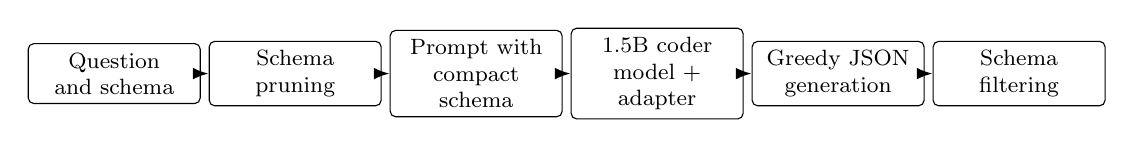
\begin{tikzpicture}[
  node distance=0.10cm,
  box/.style={draw, rounded corners=2pt, align=center, minimum height=0.72cm,
              text width=1.95cm, font=\footnotesize},
  arr/.style={-{Latex[length=2mm]}, thick}
]
\node[box] (input) {Question\\and schema};
\node[box, right=of input] (prune) {Schema\\pruning};
\node[box, right=of prune] (prompt) {Prompt with\\compact schema};
\node[box, right=of prompt] (model) {1.5B coder\\model + adapter};
\node[box, right=of model] (json) {Greedy JSON\\generation};
\node[box, right=of json] (filter) {Schema\\filtering};
\draw[arr] (input) -- (prune);
\draw[arr] (prune) -- (prompt);
\draw[arr] (prompt) -- (model);
\draw[arr] (model) -- (json);
\draw[arr] (json) -- (filter);
\end{tikzpicture}
}
\caption{Final inference pipeline. Training uses the same prompt format, but supervises only the answer tokens.}
\label{fig:pipeline}
\end{figure}

Each part of the final configuration has a specific role. The coder base model provides better
identifier and SQL-like symbol handling than the general 1.5B instruction model. The LoRA adapter
keeps the trainable artifact small enough to submit and load locally. The 4-bit QLoRA-style load
keeps training within the GPU memory budget while still updating the adapter. The pruned schema
reduces distractor columns, the database-balanced data prevents very small schemas from being
ignored, and completion-only training makes the model spend its capacity on the answer rather than
on reconstructing the prompt. The schema filter at the end improves precision by removing invalid
identifiers, but it does not invent missing links.

Training used RapidFire AI's supervised fine-tuning workflow with rank 16, alpha 32, and dropout
0.05 for the adapter \cite{hu2021lora,dettmers2023qlora}. Optimization used batch size 1, gradient
accumulation 8, cosine learning-rate scheduling, 5\% warmup, BF16 computation, learning rate
\(8.5\times 10^{-5}\), maximum length 8192, and 7 epochs. These settings were chosen after smaller
runs showed that the model needed several passes over the compact dataset, but that higher learning
rates and larger adapters could overfit or destabilize column prediction.

The prompt asks for only the tables and columns that the SQL query would reference. It explicitly
states the JSON output contract and the convention that table-only references, such as count queries,
should include the table with an empty column list. I did not use few-shot examples in the final prompt;
with the pruned schema, examples consumed context without improving validation performance.

Generation is greedy and deterministic. After generation, the predicted JSON is parsed and checked
against the database schema. Unknown tables and columns are removed, duplicate columns are
collapsed, and valid names are restored to the schema's original casing. This post-processing is
conservative: it prevents hallucinated identifiers from hurting precision, but it does not add identifiers
that the model failed to predict.

This distinction is important for the reported results. The schema filter improves output validity and
removes obvious false positives, but it is not an answer-repair system. If the model misses a join key
or predicts a broad table without the needed measure column, the post-processing step leaves that
mistake in place. Most remaining errors therefore reflect the trained model's column-selection ability,
not a mismatch between generated spelling and schema spelling.

\section{Experimentation Methodology}

I used RapidFire AI to run and compare supervised fine-tuning configurations. The evaluation loop was
kept fixed across runs: train an adapter, generate predictions on the held-out development questions,
and score them with the released set-based evaluator. The reported overall score is the average of
the table-level and column-level scores.

The search was organized as a sequence of decisions rather than as one large random sweep. The
starting point was the base model without fine-tuning, which measured how much the public model
could do from the prompt alone. After that, I added supervised fine-tuning and changed only the loss
format, then changed the schema context, then changed the data distribution, then switched the base
model, and finally tuned the learning rate, epochs, and adapter size around the best family. This made
the path to the final run interpretable instead of just selecting the best number from a table.

\begin{table}[H]
\centering
\caption{Representative configurations on the released validation split. Each row changes at least one training, data, or model choice.}
\label{tab:configs}
\resizebox{\textwidth}{!}{%
\begin{tabular}{llllrrr}
\toprule
Run & Base model & Data and schema setting & Training setting & Table & Column & Overall \\
\midrule
No SFT & Qwen2.5 1.5B & full schema & no adapter & 0.4113 & 0.2579 & 0.3346 \\
Completion only & Qwen2.5 1.5B & full schema & rank 16, alpha 16, 2 epochs, lr \(2e{-4}\) & 0.6523 & 0.4729 & 0.5626 \\
Pruned schema & Qwen2.5 1.5B & pruned schema & rank 16, alpha 16, 4 epochs, lr \(2e{-4}\) & 0.7049 & 0.5644 & 0.6347 \\
Balanced to 18 & Qwen2.5 1.5B & pruned, database target 18 & rank 16, alpha 16, 4 epochs & 0.7249 & 0.5511 & 0.6380 \\
Balanced to 12 & Qwen2.5 1.5B & pruned, database target 12 & rank 16, alpha 16, 4 epochs & 0.7254 & 0.5819 & 0.6536 \\
Coder model & Qwen2.5-Coder 1.5B & pruned, database target 12 & rank 16, alpha 32, 6 epochs, lr \(1e{-4}\) & 0.7524 & 0.5945 & 0.6735 \\
Lower learning rate & Qwen2.5-Coder 1.5B & pruned, database target 12 & 7 epochs, lr \(7.5e{-5}\) & 0.7621 & 0.5952 & 0.6787 \\
Final run & Qwen2.5-Coder 1.5B & pruned, database target 12 & 7 epochs, lr \(8.5e{-5}\) & \textbf{0.7753} & \textbf{0.5985} & \textbf{0.6869} \\
Higher learning rate & Qwen2.5-Coder 1.5B & pruned, database target 12 & 7 epochs, lr \(9e{-5}\) & 0.7351 & 0.5711 & 0.6531 \\
Larger adapter & Qwen2.5-Coder 1.5B & pruned, database target 12 & rank 32, alpha 64, 7 epochs & 0.7530 & 0.5916 & 0.6723 \\
Complex-row repeat & Qwen2.5 1.5B & repeat rows with many links & rank 16, alpha 16, 4 epochs & 0.7393 & 0.5880 & 0.6636 \\
Alternative coder & DeepSeek-Coder 1.3B & pruned, database target 12 & same final recipe & 0.7138 & 0.4831 & 0.5984 \\
\bottomrule
\end{tabular}}
\end{table}

These runs cover more than the required eight distinct configurations and show the transition from
the base model to the final system: no SFT scored 0.3346; completion-only SFT raised it to 0.5626;
schema pruning reached 0.6347; database balancing reached 0.6536; the coder base reached 0.6735;
and the final local learning-rate search reached 0.6869. RapidFire was useful because these runs used
the same training and logging path, so the differences were attributable to the intended configuration
changes rather than to separate scripts.

\section{Results and Analysis}
\enlargethispage{2\baselineskip}

The no-training baseline was weak. It often produced extra tables, invalid JSON, or plausible columns
under the wrong table. After schema filtering, its overall score was 0.3346. This matched the project
motivation: at this size, the base model is not reliable enough for schema linking without task-specific
training.

Completion-only fine-tuning was the first major improvement, raising the score to 0.5626. This was
mainly a format and discipline gain. The model learned to emit the answer object directly instead of
explaining itself or copying schema text. Pruning the schema raised the score again, to 0.6347, because
the model saw fewer irrelevant identifiers and made fewer column-level false positives.

Balancing the database distribution helped, but only mildly. Upsampling small databases to 12 rows
improved the pruned Qwen2.5 run from 0.6347 to 0.6536. A stronger target of 18 improved table
coverage but reduced column score, which suggests that repeated examples from small databases can
start to distort fine-grained column selection. The final setting uses balancing as a gentle correction,
not as an attempt to make every database equally frequent.

The largest later gain came from the base model. Switching to Qwen2.5-Coder-1.5B improved both
table and column metrics. This is plausible because schema linking is close to code and SQL reasoning:
the model must treat names like structured symbols and must learn when a question implies a filter,
join, aggregation, or measure column. A small search around learning rate and epoch count then
improved the score to 0.6869.

Not every training-side change helped. A larger LoRA adapter did not improve the final result, and
a slightly higher learning rate regressed noticeably. Repeating complex examples also reduced the
overall score, even though it helped some small modules, because it hurt larger domains enough to
lower the macro average. The alternative coder model trained cleanly but had much weaker column
accuracy, so base-model family mattered more than simply choosing any code model under 2B.

The final system still has a clear weakness: column recall and precision lag behind table prediction.
Many questions identify the right table but require a specific measure, condition, or join key that is
not obvious from surface words alone. With more budget, I would focus on training data for these
hard column patterns, especially repeated NTSB column families and low-resource SAP modules. I
would also test schema context with type or foreign-key hints, but only after controlling prompt length
so that the model is not distracted by a full schema dump.

The most useful lesson from the experiments is that the training recipe and the data view interact.
Longer context did not automatically help, because extra schema tokens increased the number of
reasonable-looking but wrong columns. More repetition also did not automatically help, because the
macro score punishes shifts that improve a few small databases while degrading larger ones. The final
model is not the most complex system I tried; it is the setting where the schema view, data balance,
base model, and optimization were all aligned with the structured-output objective.

\section{AI Tools Statement}

AI tools were used as coding, debugging, experiment-organization, and writing aids: inspecting
project files, organizing commands, summarizing results for experiment runs, and editing
report/README wording. The experiments, scores, and submitted adapter come from local project
runs and the released evaluator.

\begin{thebibliography}{9}
\bibitem{snails}
Kyle Luoma and Abhinav Kumar.
\newblock SNAILS: Schema Naming Assessments for Improved LLM-Based SQL Inference.
\newblock Proc. ACM SIGMOD, 2025.

\bibitem{rapidfireai}
RapidFire AI.
\newblock RapidFire AI.
\newblock \url{https://www.rapidfire.ai/}.

\bibitem{hu2021lora}
Edward J. Hu, Yelong Shen, Phillip Wallis, Zeyuan Allen-Zhu, Yuanzhi Li, Shean Wang, Lu Wang, and Weizhu Chen.
\newblock LoRA: Low-rank adaptation of large language models.
\newblock arXiv:2106.09685, 2021.

\bibitem{dettmers2023qlora}
Tim Dettmers, Artidoro Pagnoni, Ari Holtzman, and Luke Zettlemoyer.
\newblock QLoRA: Efficient finetuning of quantized LLMs.
\newblock arXiv:2305.14314, 2023.

\end{thebibliography}

\end{document}
